
%%%%%%%%%%%%%%%%%%%%%%%%%%%%%%%%%%%%%%%%%%%%%%%%%%%%%%%%%%%%%%%%%%%%
\section{DAQ Design}
\label{sec:fdsp-daq-design}

\metainfo{16 Pages}


%%%%%%%%%%%%%%%%%%%%%%%%%%%%%%%%%%%
\subsection{Overview (Giles Barr)}
\label{sec:fdsp-daq-ltr}

Here we describe the overall readout and data acquistion
strategy. This will include the high-level data flow diagram,
(Figure~\ref{fig:daq-readout-buffering-baseline} may be sufficient)
which is divided in functional boxes, each of which are described in
turn in the sections below.

%%%%%%%%%%%%%%%%%%%%%%%%%%%%%%%%%%%
\subsection{Local Readout \& Buffering (Giles Barr \& Giovanna Miotto \& Brett Viren)}
\label{sec:fdsp-daq-ltr}

\metainfo{Describe how the data is received from the detector electronics, and buffered while awaiting a trigger decision, together with any processing that affects stored data.  The starting point is data incoming from the WIBs and the end point is corresponding data sitting in memory ready for event building. }

Figure~\ref{fig:daq-readout-buffering-baseline} illustrates the local
readout and buffering data flow in the context of a single APA.  

\begin{dunefigure}[Baseline Readout and Buffering]{fig:daq-readout-buffering-baseline}
  {Illustration of data flow for two out of 150 APAs in the
    Single-Phase module. 
    It shows the Cold Electronics WIB-RCE connections which send one
    half of one APA face to each RCE. 
    The data and L0 trigger primitives the RCEs are received by a
    single FELIX host. 
    The data is buffered into RAM and the trigger primitives are sent
    to the Module Trigger Logic unit (MTL) and sent to the Global
    Trigger Logic unit (not shown). 
    Nominal (non-dump) trigger commands are delivered to the Event
    Builder which polls the selector on the appropriate FELIX host for
    the requested data.
    The MTL sends special SNB-dump trigger commands directly to the
    Front-End Readout hardware so that it may initiate a full-stream
    dump to local storage. 
    This dump is then sent out over Ethernet to a special SNB Event
    builder. 
    Both types of event builders finally save triggered data to file
    on the offline buffer disk.}
% This PDF is made from the .dot of the same name.
\includegraphics[width=0.8\textwidth]{daq-readout-buffering-baseline.pdf}%
\end{dunefigure}


%%%%%%%%%%%%%%%%%%%%%%%%%%%%%%%%%%%
\subsection{Local Trigger Primitive Generation (Josh Klein \& J.J. Russel \& Brett Viren \& DP Expert?)}
\label{sec:fdsp-daq-ltr}

\fixme{Below are from slides bv may show at the Jan WS.  Content copied here and now as a starting point.}

The TPC data is used to generate \textit{trigger primitive messages}
(TPM) local to each APA and which summarize the activity recently
sensed by their connected conductors.  These TPMs are emited from each
APA DAQ Front End and become fodder for later determining
\textit{trigger command messages} (TCM) as described in
Section~\ref{sec:fdsp-daq-sel}.

Only the 480 collection channels associated with each APA face are
used for forming TCMs.  Reasons for this reduction include the fact
that collection channels:

\begin{itemize}
\item have higher signal to noise ratio compared to induction channels.
\item fully and independently are sensitive to each APA face.
\item have unipolar signals that directly give an approximate measure
  of ionization charge without costly field response deconvolution
  computation.
\item can be divided into smaller groups defined by natural hardware
  boundaries for parallel processing.
  % fixme: do we need a statement about efficiency here?
\end{itemize}


Figure~\ref{fig:daq-overview} illustrates the connectivity between the
four connectors on each of the five WIBs and the DAQ APA Front End.
The data is received from 80 1 Gbps fiber optical links by four
Reconfigurable Computing Elements (RCE) in the ACTA Cluster On Board
(COB) system. \fixme{Matt: help!  Each RCE consists of a ....}

The pattern of connectivity between WIBs and RCEs results in the data
from the collection channels covering one half of one APA face being
received by each RCE.  Each RCE has two primary functions.  The first
is transmission of all data as described in
Section~\ref{sec:fdsp-daq-hlt}.  The second is to produce TPMs from
its portion of the collection channel data.

The TPMs are produced from a \textit{trigger primitive production
  pipeline} of algorithms.  These algorithms still require development
but can be broadly described.   

\begin{enumerate}
\item On a per channel basis calculate a rolling baseline and RMS that
  characterizes recent samples minimal influence from ionization
  signal.
\item Locate contiguous ADC samples that go above a threshold which is
  defined in terms of the baseline and RMS.
\item Emit their time bounds and total charge as a $ROI_{ch}$ TPM.
\end{enumerate}

These $ROI_{ch}$ TPM represent some possible activity occurring
somewhere in the LAr within a $\pm$\SI{2.5}{\mm} strip that extends in
time by the ROI time bounds.  Depending on the threshold set, these
TPMs may be numerous due to \Ar39 decays and noise fluctuations.
Further processing must be done with more global information.  This
may be done as part of the Module Trigger Logic (MTL) as described in
Section~\ref{sec:fdsp-daq-sel} or it may be done immediately in the
RCE pipeline.  Strategies to summarize these detailed TPM into fewer
TPMs include:

\begin{enumerate}
\item Pad each $ROI_{ch}$ in a channel by a fixed amount in order to
  anticipate their use later as defining readout (eg, long enough to
  account for inter-plane drift times (\SI{6.25}{\micro\second}) and
  induction signal extents ($\sim$\SI{100}{\micro\second}).
\item Form the union of ROI across all channels observed by a given RCE.
\item Merge subsequent ROI which are separated by some small time
  interval.
\end{enumerate}

If the Single-Phase detector module generates excess noise, such as
that from RF emission picked up coherently across some group of
channel, it must be mitigated at the start of the pipeline and will
likely require additional computational resources.  Some ideas to
respond to this scenario include....\fixme{Ideas?}.



%%%%%%%%%%%%%%%%%%%%%%%%%%%%%%%%%%%
\subsection{Dataflow, Trigger and Event Builder (Giles Barr \& Josh Klein \& Giovanna Miotto \& Kurt Biery \& Brett Viren)}
\label{sec:fdsp-daq-hlt}

\metainfo{Describe the dataflow {\it infrastructure}. This should cover transport of data and trigger information, infrastructure for generating local and global trigger commands (but not their algorithms, that's next), as well as what happens to the data once a trigger is generated (ie. event building).
Figure~\ref{fig:daq-readout-buffering-baseline} may be referenced}


%%%%%%%%%%%%%%%%%%%%%%%%%%%%%%%%%%%
\subsection{Data Selection Algorithms (Josh Klein \& Brett Viren)}
\label{sec:fdsp-daq-sel}

%This section describes the strategy for using the trigger/dataflow infrastructure, with example algorithms.

	Data Selection will follow a hierarchical design, beginning with local,
APA Level triggers, Module (10 ktonne) Level triggers, and Global
(Detector-wide) triggers. A high-level trigger (HLT) may also be active within
the Module Level trigger.  The hierarchical approach is both natural from a
design standpoint, as well as allowing for vertical slice testing and
partitioning during commissioning of the system.

	As discussed above, trigger primitives will be generated in the RCEs
from the data stream for each collection wires.  The trigger primitives will be
summary information for each collection wire, such as the time of any
threshold-crossing pulse, its integral charge, and time over threshold.  A
collection wire with a non-null trigger primitive is said to be ``hit.''  These
trigger primitives are then passed, along with the full data stream, to the
FELIX boards and their hosts, each of which handles channels from a small
number of APAs (likely two).  An APA Level trigger decision is passed upward to
a Module Level trigger, which arbirtrates between various trigger types,
determining whether a given APA Level trigger is a valid Module Trigger and
whether there are other triggers that have a higher priority in any given slice
of time.  At this level, a more sophisticated high-level trigger (HLT) may also
be employed, which will allow a reduction in trigger rate from various
backrounds, including instrumental backgrounds, if needed. 

	A valid Module Level single-interaction trigger sends trigger commands
back to the FELIX hosts telling them which slice of time should be saved under
the particular trigger header.  At the start of DUNE data taking, it is
anticipated that for any given single-interaction trigger (a cosmic ray track,
for example) waveforms for all wires will be recorded for a full 5.4~ms
``readout window.'' Such an approach is clearly very conservative, but it
ensures that associated low-energy physics (such as neutron captures from
neutrons produced by neutrino interactions or cosmic rays) will be recorded
without any need to fine-tune APA-level triggering, and will not depend on
the noise environment across the APAs. In addition, the 5.4~ms readout window
ensures that regardless of when a given even causes a trigger, the entire track
is recorded.  We anticipate, however, that as we gain experience running DUNE
the overall data volume will reduced either by writing out data from only a
subset of APAs for any given track, and possibly reducing the size of the
readout window.

	Other trigger streams---calibrations, random triggers, and prescales of
various trigger thresholds, will also be generated at the Module Level, and
filtering and compression can be applied based upon the trigger stream. For
example, a large fraction of random triggers may have their waveforms
zero-suppressed, reducing the data volume substantially, as the dominant data
source for these will be $^{39}$Ar events. Additional signal-processing can
also be done on particular trigger streams if needed and if the processing is
available, such as fast analyses of calibration data.

       At the Module Level, a decision can also be made on whether a series of
interactions are consistent with a supernova burst.  If the number of APA Level
triggers exceeds a threshold for the number of such events in a given time, a
trigger command is sent from the Module Level back to the RCEs, which store up
to 10 seconds of unsuppressed, full waveform data.  That full waveform is then
written out as a separate trigger stream for fast analysis by the supernova
working group, perhaps as an automated process.  In addition, the Module Level
passes information about APA Level triggers up to a detector-wide Global
Trigger, which can decide whether, integrated across all modules, enough APAs
have detected interactions to qualify for a supernova burst even if within a
particular module the threshold is not exceeded. Trigger commands from the
Global Trigger Level are passed downward to RCEs in the same way as any Module
Level supernova burst trigger would be; at the Module Level, a Global Trigger
looks like just one more ``external'' trigger input.

	APA-Level Trigger decisions will be made within each FELIX
host.  The trigger decision will be based on the number of adjacent wires hit
in a given APA within a narrow time window (roughly 100$\mu$s), the total
charge on these adjacent wires (or any wire with a non-null trigger primitive),
and possibly the time-over-threshold for collection wires with hits. Our
studies show that even for low-energy events (roughly 10-20 MeV) the reduction
in radiological backgrounds is extremely high with such criteria. The
highest-rate background, $^{39}$Ar, which has a decay rate of 10 MBq within a
10 ktonne volume of argon, has an endpoint of 500 keV and requires significant
pileup in both space and time to get near a 10 MeV threshold. Other important
background sources are $^{42}$Ar, which has a 3.5 MeV endpoint and a decay rate
of 1 kBq, and $^{222}$Rn which has a decay rate of XXXX and decays via a
highly-quenched $\alpha$ of 5.5 MeV.  The radon decays to $^{218}$Po which
a few minutes later leads to a quenched $\alpha$ of 6 MeV, and ultimately a
$^{214}$Bi daughter (many minutes later) which has a $\beta$ decay with
endpoint near 3.5 MeV.  The $\alpha$ ranges are short and will hit at most a
few collection wires, but the charge deposit can be large, and therefore the
charge threshold will have to be well above the $\alpha$ deposits plus any
pileup from $^{39}$Ar and noise.

	At the APA Level, two kinds of local trigger decisions can be made. One
is a ``high-energy'' trigger, that indicates that within a given APA a
candidate event with energy more than 10 MeV has been found. The thresholds in
hit wires, total charge, and time-over-threshold, will be optimized for at
least 50\% efficiency at this threshold, with efficiency increasing to 100\%
via a turn-on curve that ensures at least 90\% efficiency at 20 MeV.  
A second APA-level trigger will be optimized for low-energy events, between 
5~MeV and 10 MeV. These low-energy APA triggers will not by themselves generate
valid  Module Level triggers, but rather be used at the Module Level to
determine whether a burst of events across many APAs is consistent with a
supernova.

	The Module Level takes as input both APA Level triggers (both
low-energy and high-energy), as well as external trigger sources, such as the
Global (detector-wide) trigger, external triggers such as SNEWS, and
information about the time of a Fermilab Beam spill.  The Module Level will
also generate internal triggers, such as random triggers and calibration
triggers (for example, telling a laser system to fire at a prescribed time). 
In addition, at the Module Level prescales of all trigger types that normally
would not generate a Module Level will be made. For example, a single
low-energy trigger does not cause a Module Level trigger on its own, but at
some large prescale fraction it could be accepted.

	The Module Level is responsible also for checking candidate triggers
against the current Run Control trigger mask: in some runs, for example, we
may decide that only random triggers are accepted, or that certain APA trigger
candidates should not be accepted because those APAs are noisy or misbehaving
in some way.  In addition, the Module Level will count low-energy trigger
candidates from the APAs and, based upon the number and distribution of those
triggers in a long time interval (e.g., 10 seconds), decide to generate a
supernova burst trigger command. The trigger logic for a supernova burst will
be optimized to accept at least 90\% of all Milky Way supernovae, and our
studies of simple low-energy trigger criteria show that we can likely do much
better than that.  

	The HLT can also be applied at this level, particularly if there are
unexpectedly higher rates from instrumental or low-energy backgrounds, that
require some level of reconstruction or pattern recognition.  An HLT might also
allow for efficency triggering on lower-energy single interactions, or allow
for better sensitivity for supernovae beyond the Milky Way, by employing a
weighting scheme to individual APA Level trigger candidates---higher-energy
trigger candidates receiving higher weights. Thus, for example, two APA Level
trigger candidates consistent with 10 MeV interactions in 10 seconds might be
enough to create a supernova burst candidate trigger, while 100 5 MeV APA Level
trigger candiates in 10 seconds might not. Lastly, the HLT can allow for
dynamic thresholding; for example, if a trigger appears to be a cosmic-ray
muon, the threshold for single interactions can be lowered (and possibly
prescaled) for a short time after that to identify spallation products. In
addition, the HLT could allow for a dynamic threshold after a supernova burst,
to extend sensitivity beyond the 10 s readout buffer, while not increasing the
data volume associated with supernova burst candidates linearly. 

All low-energy trigger candidates are also passed upwards to the Global trigger
level, which can integrate the APA level trigger across all 10 ktonne modules
and determine if enough APAs have trigger candidates that a supernova burst may
be occuring. This approach increases the sensitivity to trigger bursts by a
factor of four (for 40 ktonnes), thus extending the burst sensitivity to a
distance twice as far as for a single 10 ktonne module. 

	The Module Level is also responsible for creating a trigger header that
includes a global timestamp for the trigger, and information on what type of
trigger was created. A log of all APA Level trigger candidates will also be
kept, whether or not they are part of a Module Trigger. The Module Level also
generates the commands that either tell the FELIX hosts to write out a 5.4~ms
slice of their buffer (providing the start and end times to the FELIX hosts)
as well as the commands that tell the RCEs to dump their 10 s unsuppressed
``supernova'' buffer.  If a supernova burst trigger is created at the Global
trigger level, a trigger command is passed back down to the Module Level, which
then passes that on to the RCEs for readout of the long (10 s) unsuppressed
buffer, the same way it would if a supernova burst is detected at the Module
Level. 

	


%\metainfo{Describe Module Trigger Logic and Global Trigger Logic.
%  Describe creation of Trigger Command Messages (TCM) from TPMs.
%  Included external sources of TPMs such as SNEWS, Fermilab Beam,
%  testing triggers, periodic triggers, calibration triggers.}
%
%\metainfo{Here should go the assumptions that went into the thinking
%  for Josh's event category data volumes.  It can include discussion
%  of tighter selection criteria for ``cosmics'' such as Phil's
%  distribution of number of APAs hit by cosmics and arguments for
%  something less than 2+ drift time readouts.}

%
% %%%%%%%%%%%%%%%%%%%%%%%%%%%%%%%%%%%
% \subsection{High-Level Trigger}
% \label{sec:fdsp-daq-eb}
%
% Data selection after event building.
%

\subsection{Timing \& Synchronization (David Cussans \& Kostas Manolopoulos)}
\label{sec:fdsp-daq-timing}

%Describe the generation of timing/synchronisation signals and and distribution to the detectors.

The DUNE Single Phase detectors use a development of the protoDUNE timing system. Synchronization messages are transmitted over a serial data stream with the clock embedded in the data. The format is described in DUNE DocDB-1651. Figure \ref{fig:daq-readout-sp-timing} shows the overall arrangement of components within the Single Phase Timing System(SPTS).

\begin{dunefigure}[Arrangement of components in Single Phase Timing System]{fig:daq-readout-sp-timing}
  {Illustration of the components in the Single Phase Timing System. \fixme{Replace this protoDUNE SP timing system diagram with a DUNE diagram.}}
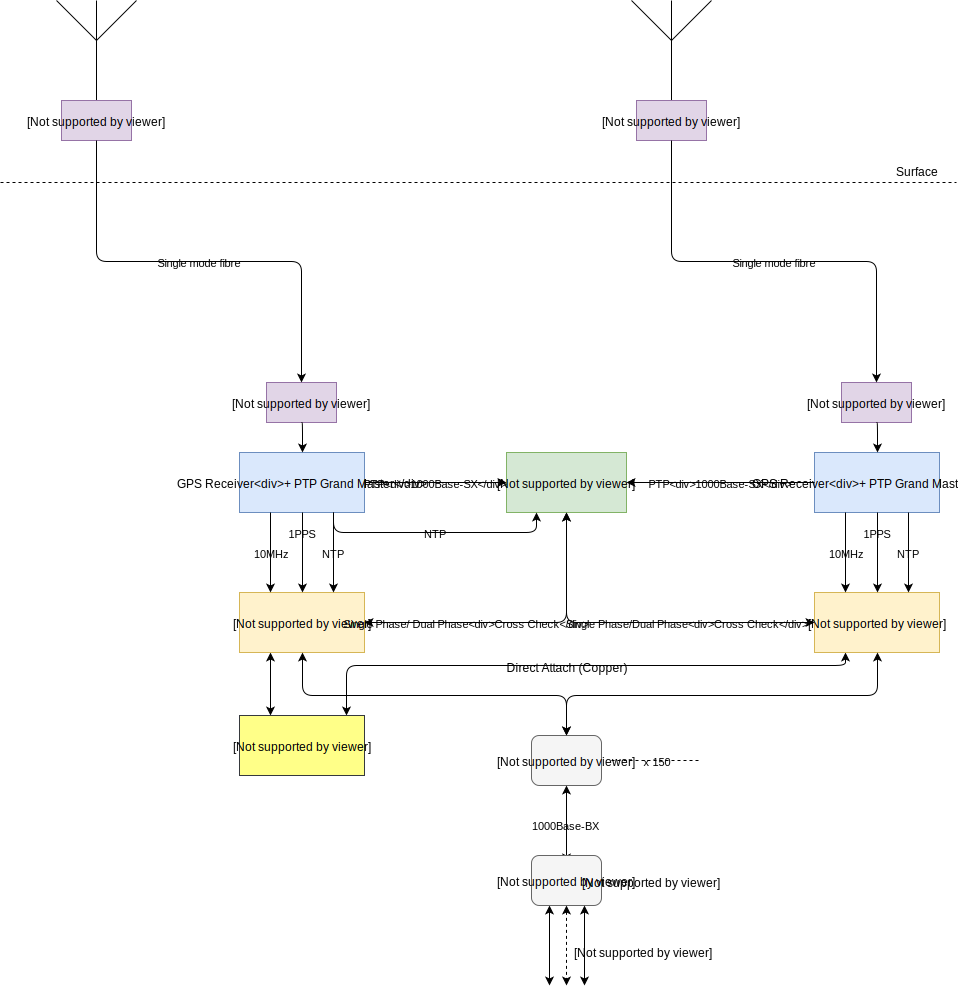
\includegraphics[width=0.8\textwidth]{DUNE_Timing_overall.pdf}
\end{dunefigure}



%%%%%%%%%%%%%%%%%%%%%%%%%%%%%%%%%%%
\subsection{Computing \& Network Infrastructure (Kurt Biery \& Babak Abi)}
\label{sec:fdsp-daq-infra}

Describes the infrastructure that will support the software components described above.

%%%%%%%%%%%%%%%%%%%%%%%%%%%%%%%%%%%
\subsection{Run Control \& Monitoring (Giovanna Miotto \& Jingbo Wang}
\label{sec:fdsp-daq-tcm}

Describe how the system is controlled and monitored.

